% Nejprve uvedeme tridu dokumentu s volbami
\documentclass[czech,bachelor,public,dept460,male,cpdeclaration,twoside]{diploma}
% Dalsi doplnujici baliky maker
\usepackage{subfig}		% makra pro "podobrazky" a "podtabulky"
\usepackage{tikz}		% makra pro kresleni

% Zadame pozadovane vstupy pro generovani titulnich stran.
\ThesisAuthor{Lukáš Hanusek}

\CzechThesisTitle{Tvorba aplikace pro simulaci problémů v databázovém systému}

\EnglishThesisTitle{Application for Simulation of Database Problems}

\SubmissionDate{1. dubna 2019}

\Thanks{Rád bych zde poděkoval vedoucímu bakalářské práce, kterým je doc. Ing. Radim Bača, Ph.D., za jeho cenné rady během vytváření výsledné aplikace.}

% Pokud nechceme nikomu dekovat makro zapoznamkujeme.
%\Thanks{Rád bych na tomto místě poděkoval všem, kteří mi s prací pomohli, protože bez nich by tato práce nevznikla.}

% Zadame cestu a jmeno souboru ci nekolika souboru s digitalizovanou podobou zadani prace.
% Pokud toto makro zapoznamkujeme sazi se stranka s upozornenim.
\ThesisAssignmentImagePath{Figures/Assignment}

% Zadame soubor s digitalizovanou podobou prohlaseni autora zaverecne prace.
% Pokud toto makro zapoznamkujeme sazi se cisty text prohlaseni.
%\AuthorDeclarationImageFile{Figures/AuthorDeclaration.jpg}


% Zadame soubor s digitalizovanou podobou souhlasu spolupracujici prav. nebo fyz. osoby.
% Pokud toto makro zapoznamkujeme sazi se cisty text souhlasu.
%\CooperatingPersonsDeclarationImageFile{Figures/CoopPersonDeclaration.jpg}


% řazeno podle abecedy nikoliv podle výskytů v textu
\AddAcronym{API}{Application Programming Interface}
\AddAcronym{CSV}{Comma-separated values}
\AddAcronym{DB}{Databáze}
\AddAcronym{DBMS}{Database Management system (Systém řízení báze dat)}
\AddAcronym{IDE}{Integrated Development Environment}
\AddAcronym{JAXB}{Java Architecture for XML Binding (\ref{jabx})}
\AddAcronym{JDBC}{Java Database Connectivity (\ref{jdbc})}
\AddAcronym{JRE}{Java Runtime Environment}
\AddAcronym{JVM}{Java Virtual Machine}
\AddAcronym{SQL}{Structured Query Language - Dotazovací jazyk pro manipulaci s daty na databázovém systému založeném na SQL}
\AddAcronym{SŘBD}{Systém řízení báze dat}
\AddAcronym{UML}{Unified Modeling Language}
\AddAcronym{XML}{eXtensible Markup Language}




\CzechAbstract{Tato bakalářská práce se zabývá simulováním problémů, které mohou nastat na databázovém serveru. Cílem práce je vytvořit aplikaci, která umožní definovat způsob vytížení databáze a simulovat reálný provoz. Správce databázového serveru tak má možnost vyzkoušet a odladit problémy, ještě před tím, než se databázový server uvede do reálného provozu.}

\CzechKeywords{SQL, databáze, simulace vytížení, validace SQL}

\EnglishAbstract{The purpose of this bachelor thesis is to simulate problems that could take place on a production database server. The objective is to create an application that will allow database administrators to specify the type of workload and simulate real database traffic. This way database administrators can find and solve performance problems that might come up during the test before using the database in a production environment.}

\EnglishKeywords{SQL, database, workload simulation, SQL validation}

% Zacatek dokumentu
\begin{document}

% Nechame vysazet titulni strany.
\MakeTitlePages


% A nasleduje text zaverecne prace.
\section{Úvod}
Databáze dnes stojí v pozadí téměř každé webové stránky, počítačového programu nebo mobilní aplikace. Úkolem databáze je ukládat, načítat, třídit, seskupovat a filtrovat všechna potřebná data pro běh dané aplikace, zajistit jejich perzistenci, zabezpečení a spravovat k datům přístup. \par
Cílem práce je vytvořit aplikaci pro simulaci problémů v databázovém systému, aplikace bude simulovat reálné situace, ve kterých se může databáze nacházet. Správce databáze tak může odhalit chyby nebo případné nedostatky ještě před nasazením systému do produkčního prostředí a předejít výpadkům dostupnosti databáze. \par
Mezi hlavní důvody, proč používat pro ukládání dat databázi, na místo ukládání dat přímo do souborů, patří především dostupnost a vzdálený přístup k datům z jiných zařízení, které databázové systémy nabízí. Dále pak rychlost přístupu k datům a vyhledávání. Pokud máme například data uložena v souboru na disku a potřebujeme tyto data zobrazit na jiném zařízení, nezbývá nic jiného, než celý soubor přenést na druhé zařízení, pokud ale potřebujeme zobrazit jen určitou část dat, pak zbytek dat v souboru bylo přenášeno zbytečně. S tím souvisí problém při vyhledávání, pokud potřebujeme najít pouze jeden záznam, nezbývá nic jiného, než sekvenčně procházet všechny záznamy v souboru, dokud nenarazíme na ten, který hledáme. Při ukládání dat do databáze máme možnost z databáze vybrat a zobrazit pouze ty záznamy, které potřebujeme a není potřeba kopírovat nebo přenášet po síti všechny, tím odpadá nutnost vyhledávání v datech na koncovém zařízení, kde data zobrazujeme, vyhledávání vyřeší databáze a při správném nastavení indexů s mnohem vyšší efektivitou, než při sekvenčním hledání na koncovém zařízení. \par
Tato práce se zabývá databázemi založených na SQL, veškeré operace nad databází tedy probíhají pomocí SQL. Aplikace, tvořena v rámci této práce, používá k simulaci reálného provozu na databázi sekvenci uživatelem definovaných SQL dotazů, které jsou na databázi zasílané v definovaném pořadí s určitým intervalem. Aplikace průběžně měří a zobrazuje výsledky testu.\par
Při ukládání dat do databáze předpokládáme, že data musí být přístupná nepřetržitě, a že k datům bude přistupovat více vzdálených zařízení najednou. Proto jsou databáze často provozovány na samostatném počítači, pracovní stanici nebo serveru s velmi dobrou konektivitou do sítě a záložním zdrojem energie.

\section{DBMS} \label{dbms}
\subsection{Obecné vlastnosti DBMS}
Database Management System (Systém řízení báze dat) je software pro správu dat, který umožňuje vytváření, editování, mazání a procházení dat. Mezi nejdůležitější vlastnosti každého DBMS patří skupina vlastností označována jako \textit{ACID (Atomicity (atomičnost), Consistency (konzistence), Isolation (izolace), Durability (trvalost))}.

\subsection{Jazyk SQL (Structured Query Language)}
Jazyk SQL je doménově specifický jazyk standardizován organizací ISO (International Organization for Standardization) pod označením ISO/IEC 9075:2016. Poslední verze standardizace je z prosince 2016 \cite{sqliso}. Samotný jazyk SQL se dá rozdělit do 4 kategorií:
\begin{itemize}
  \item \textbf{Data Query Language (DQL)} slouží pro procházení a čtení dat.
  \item \textbf{Data Definition Language (DDL)} se používá pro definování datových struktur.
  \item \textbf{Data Manipulation Language (DML)} aktualizuje, maže a přidává data.
  \item \textbf{Data Control Language (DCL)} se používá pro správu přístupu k datům.
\end{itemize}

V komplexnějších DBMS nalezneme ještě 5. kategorii \textbf{Declarative Language (deklarativní jazyk)}, také označován jako \textbf{procedurální rozšíření SQL}. Procedurální rozšíření jednotlivých DBMS se liší v syntaxi a neřídí se jednotným standardem. V případě Microsoft SQL Serveru se jazyk nazývá TransactSQL (T-SQL) a v případě Oracle Databáze se jazyk jmenuje PL/SQL.


\subsection{Parametry vytížení databázového serveru}
Pod pojmem vytížení databáze se skrývá celá řada parametrů, které je potřeba monitorovat, aby bylo možné identifikovat, co nejvíce zatěžuje databázový server a zpomaluje tak jeho činnost, případně jaký postup zvolit k řešení problému. Mezi nejdůležitější parametry patří:
\begin{itemize}
  \item \textbf{Počet dotazů za vteřinu} - Počet dotazů za vteřinu je důležitý údaj, podle kterého můžeme porovnávat další parametry jako například vytížení procesoru, počet přístupů na disk nebo vytížení sítě. Toto číslo však nikdy nebude přímým ukazatelem vytížení, protože každý dotaz provádí odlišně náročné operace.
  \item \textbf{Doba zpracování dotazu} - Tento údaj je velmi důležitý, pokud monitorujeme dotazy na databázi, jejichž zpracování trvá dlouho. Můžeme tak odhalit problémy, zejména v samotném návrhu struktury databáze, nebo špatnou konstrukci SQL dotazů, které jsou na databázi zasílány.
  \item \textbf{Vytížení procesoru} - Je základní údaj, který je možné porovnávat s počtem dotazů na databázi. 
  \item \textbf{Počet přístupů na disk} - Každý správně navržený DBMS se snaží omezit počet přístupů na disk tím, že často používaná data načítá do části operační paměti nazývané jako vyrovnávací paměť. Při nedostatku operační paměti je databázový server nucen z disku opakovaně načítat stránky před vyhodnocením dotazu, které by jinak mohly být při dostatku operační paměti uloženy ve vyrovnávací paměti. Výsledkem je vysoký počet přístupů na disk a pomalý přístup k datům.
  \item \textbf{Počet SQL kompilací / rekompilací} - Pro každý SQL dotaz je na databázovém serveru sestavován plán jeho vykonání. Správně navržené aplikace by na databázový server měly posílat předem připravené SQL dotazy a za běhu aplikace zasílat na databázový server opakovaně stejně strukturované SQL dotazy jen s jinými argumenty. Protože sestavit plán vykonání dotazu je pro databázový server časově náročná operace, mělo by k sestavování docházet co nejméně. 
  \item \textbf{Vytížení sítě} - Při monitorování sítě sledujeme parametry:
  \begin{itemize}
  	\item \textbf{Délka fronty na síťovém rozhraní} - Pokud fronta na síťovém rozhraní dosahuje vysokých hodnot a kapacity linky není plně využita, může se jednat o problém s nedostatečným výkonem hardware síťového rozhraní (síťová karta).
  	\item \textbf{Rychlost odesílání / přijímaní dat} - Tento parametr je nutné porovnávat v celkovou propustností linky, kterou má databázový server k dispozici. 
  \end{itemize}
\end{itemize}


\section{Použitá technologie pro implementaci aplikace} \label{tech}

\subsection{Programovací jazyk Java}
Pro implementaci aplikace jsem zvolil programovací jazyk Java. Hlavní výhodou tohoto jazyka je přenositelnost aplikace mezi různými operačními systémy bez nutnosti úprav zdrojového kódu nebo jeho opětovného překladu. Tuto funkcionalitu zajišťuje prostředí JVM (Java Virtual Machine), které je součástí každé instalace JRE (Java Runtime Environment). Teprve v prostředí JVM dochází k překladu zkompilovaného Java byte-code na strojový kód a tak je zajištěno, že se aplikace bude chovat shodně pod různými systémy.

\subsection{JDBC (Java Database Connectivity)} \label{jdbc}
JDBC je API pro programovací jazyk Java, které definuje způsob, jak přistupovat k databázi. JDBC se používá na straně aplikace, která chce s databází komunikovat. JDBC požadavky aplikace přes JDBC API přeloží na protokol, který využívá daný databázový systém. Výhodou JDBC je, že jeho zdrojový kód je veřejně dostupný, proto si každý výrobce databázového systému může JDBC implementovat. Tím je zajištěno, že k různým databázovým systémům se přistupuje přes jednotné JDBC API.


\subsection{Knihovna JavaFX pro grafické rozhraní}
JavaFX je platforma pro tvorbu grafických uživatelských rozhraní aplikací v programovacím jazyce Java. JavaFX se liší od ostatních platforem, dostupných v základní instalaci Java Standard Edition, především tím, že grafické komponenty, jejich rozmístění a chování se definuje v odděleném souboru s příponou .FXML, tento soubor má formát XML. U ostatních Platforem jako Java AWT (Abstract Window Toolkit) nebo Swing se definují vlastnosti grafických komponent přímo v souborech se zdrojovým kódem. Každý FXML soubor definuje jedno grafické rozhraní (okno) aplikace a každý FXML soubor má přidruženou jednu třídu, která se označuje jako "Controller", který zajišťuje funkcionalitu grafických komponent. JavaFX se tak blíží návrhovému vzoru MVC (Model-View-Controller).

\subsection{SceneBuilder}
JavaFX Scene Builder je nástroj pro vytváření uživatelských grafických rozhraní pro JavaFX. Jedná se o nástroj typu "WYSIWYG", což je zkratka pro "What You See Is What You Get", přeloženo "To co vidíte, to dostanete". Nástroj SceneBuilder umožnuje grafické komponenty "přetahovat", editovat jejich parametry jako odsazení od krajů, minimální, maximální a preferovanou velikost. V prostředí SceneBuilder lze rovněž propojit grafické prvky s událostmi, jako například kliknutí na tlačítko, a nastavit odchycení této události v přidružené Controller třídě. Výstupem z tohoto programu je soubor formátu FXML, který může být načten JavaFX aplikací.
\cite{scenebuilder}

\begin{figure}[!h]\centering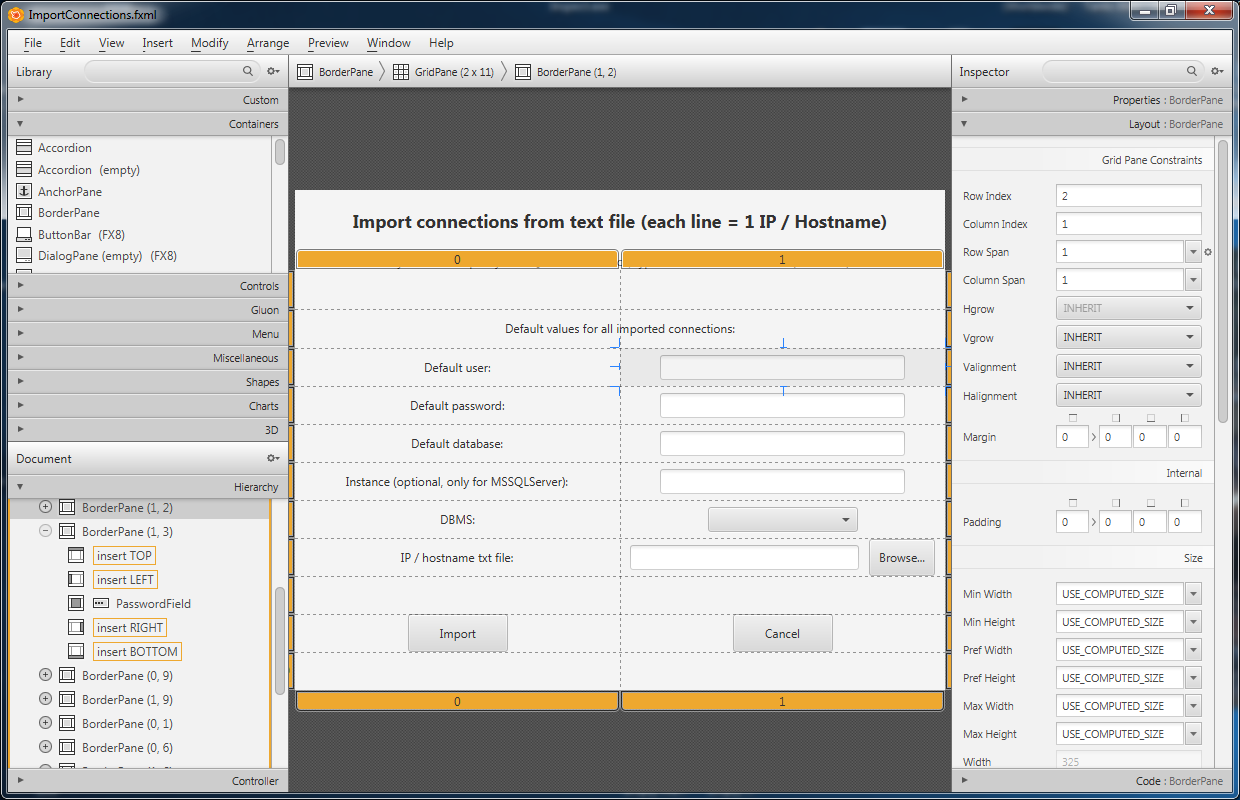
\includegraphics[width=1.0\textwidth]{Figures/SceneBuilder.png}\caption{Rozhraní nástroje SceneBuilder}
\end{figure}

\subsection{Vývojové prostředí Netbeans IDE 8.2} \label{netbeans}
NetBeans IDE byl prvním nástrojem pro vývoj Java aplikací. Projekt vznikl v České Republice jako studentský projekt v roce 1996, původně pojmenován jako Xelfi. V roce 1999 byl projekt odkoupen společností Sun Microsystems, tehdejším vývojářem programovacího jazyka Java. NetBeans se tak stal oficiálním nástrojem pro tvorbu Java aplikací. V roce 2010 byla společnost Sun Microsystems odkoupena společností Oracle. Projekt NetBeans byl dále podporován Oracle vývojáři. V roce 2016 společnost Oracle "darovala" projekt společnosti Apache Software Foundation, která převzala vývoj nástroje a stále jej vede jako open-source (veřejně dostupný zdrojový kód), nicméně při převodu projektu společnost Apache Software Foundation nezískala autorské práva ke všem součástím software NetBeans a proto jsou nové verze NetBeans pojmenovány "NetBeans IDE (incubating)", neobsahují všechny funkce a součásti, které obsahovala poslední verze NetBeans 8.2, vydaná společností Oracle. \cite{netbeans}


\section{Struktura aplikace}
Pro zajištění co největší přehlednosti zdrojového kódu je implementace aplikace je rozdělena do tří vrstev:
\begin{itemize}
  	\item \textbf{Datová vrstva} se stará o ukládání, načítání a editování perzistentních dat v aplikaci. Datová vrstva je umístěna v balíku (Java package) \textit{dbstresstest.data}. Více v sekci \ref{datalayer}.
  	\item \textbf{Prezentační vrstva} poskytuje uživatelské rozhraní aplikace, ve kterém je možno vytvářet, editovat a mazat data aplikace. Dále pak spouštět a monitorovat úlohy. Prezentační vrstva je umístěna v balíku \textit{dbstresstest.gui}. Více v sekci \ref{presentlayer}.
  	\item \textbf{Logická vrstva} zajišťuje vykonávání uživatelem spuštěných úloh, kontrolu uživatelského vstupu a komunikaci mezi datovou a prezentační vrstvou aplikace. Logická vrstva je umístěna v balíku \textit{dbstresstest.logic}. Více v sekci \ref{logiclayer}.
\end{itemize}  	
\newpage
\section{Datová vrstva} \label{datalayer}
\subsection{Diagram tříd} \label{datadiagram}
\begin{figure}[!htbp]\centering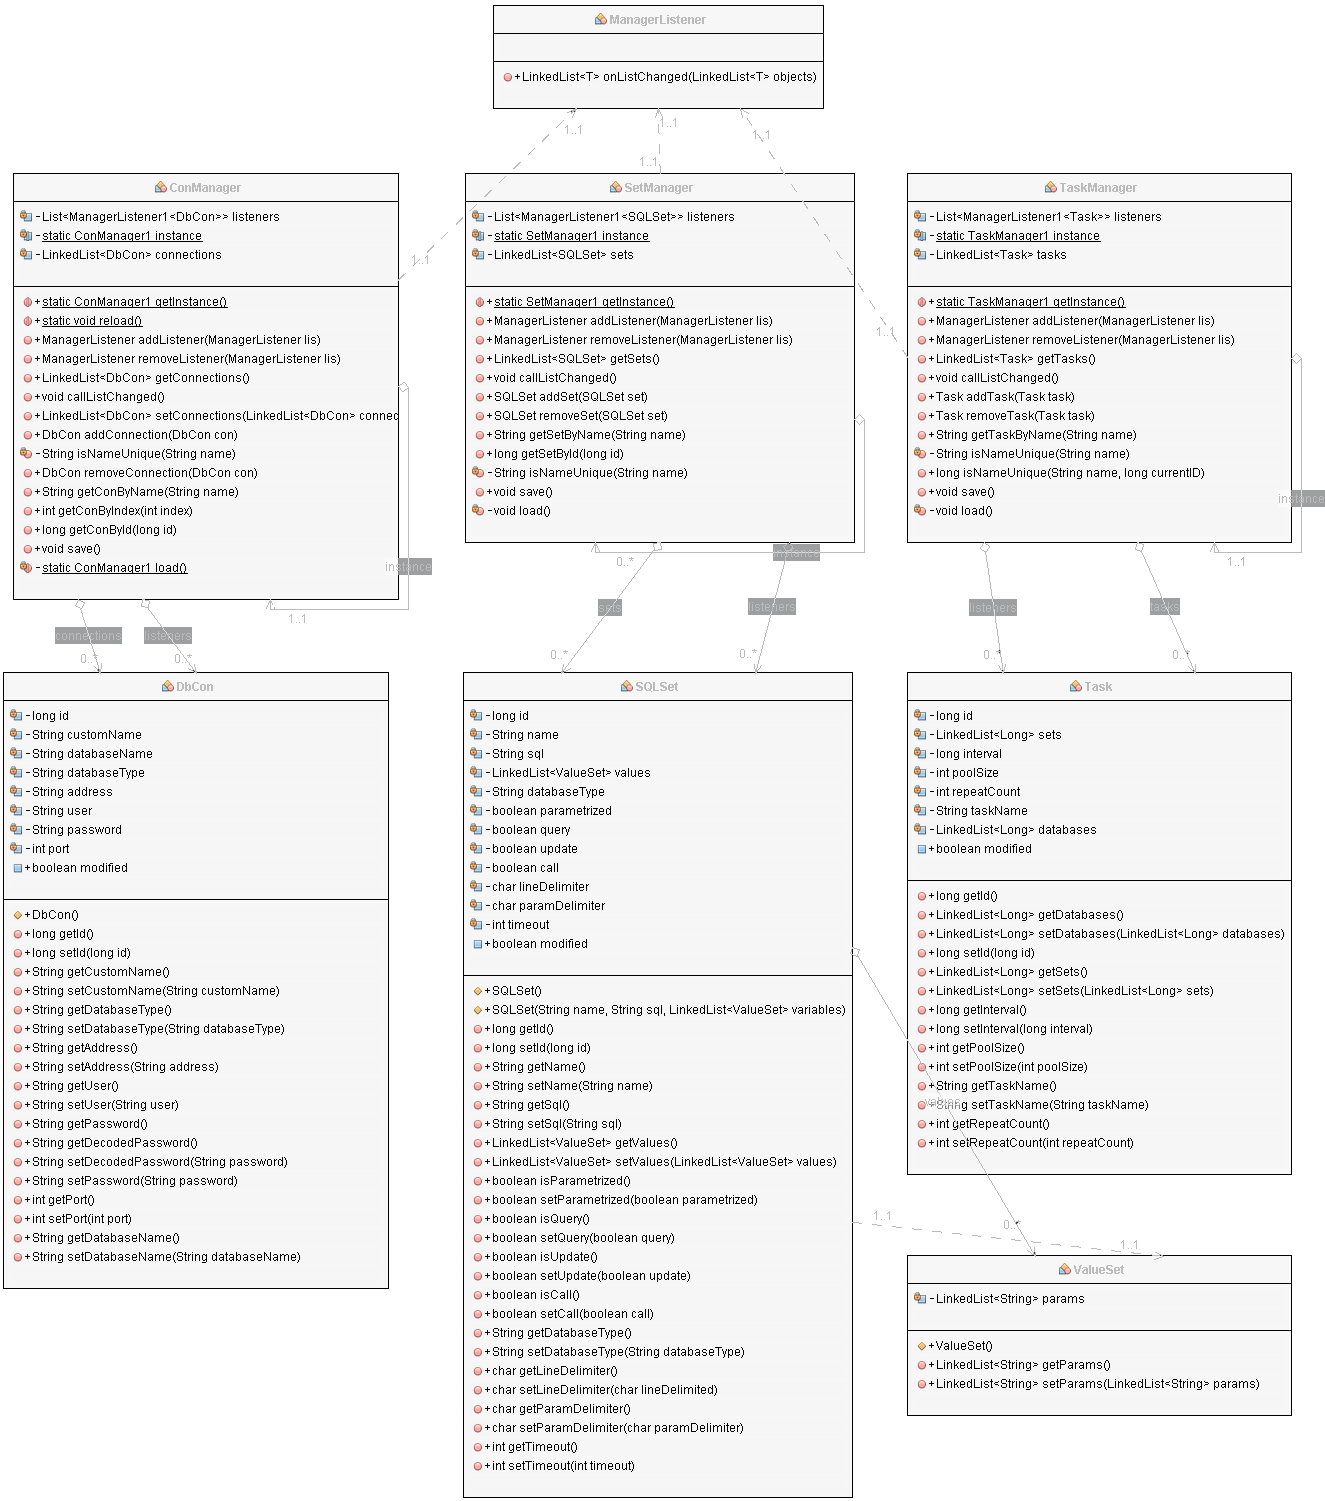
\includegraphics[width=1.0\textwidth]{Figures/DataLayerDiagram.png}\caption{UML Diagram tříd datové vrstvy aplikace}
\end{figure}
\newpage
Aplikace perzistentně ukládá tyto datové struktury:

\begin{itemize}
  \item \textbf{Údaje k připojení k databázovému serveru} - Tento typ dat je v aplikaci reprezentován třídou \textbf{\emph{DbCon}}. Načítání a ukládání objektů, vytvořených z této třídy, do perzistentního úložiště provádí třída \textbf{\emph{ConManager}} (\ref{lst:con}). Třída je realizována podle návrhového vzoru Singleton, aby bylo zaručeno, že za běhu aplikace bude existovat pouze jedna kopie dat v operační paměti aplikace. Třída \textbf{\emph{DbCon}} zapouzdřuje tyto data:
  \begin{itemize}
  	\item \textit{id} - unikátní identifikátor na logické vrstvě aplikace (\ref{logic})
  	\item \textit{customName} - unikátní jméno definované uživatelem, slouží jako identifikátor na prezentační vrstvě (\ref{prezent})
  	\item \textit{databaseName} - jméno databáze
  	\item \textit{databaseType} - rozšíření aplikace, které bude použito pro připojení k databázovému serveru
  	\item \textit{address} - adresa databázového serveru (v případě Microsoft SQL Server může~obsahovat~jméno instance)
  	\item \textit{user} - databázový uživatel
  	\item \textit{password} - heslo databázového uživatele, používá kódování Base64
  	\item \textit{port} - číslo portu databáze, hodnota 0 značí výchozí hodnotu v JDBC řadiči
  \end{itemize}
  
  \item \textbf{SQL dotazy s parametry} - Tento typ dat reprezentuje třída \textbf{\emph{SQLSet}}, tato třída dále obsahuje seznam parametrů pro SQL dotaz, reprezentován třídou \textbf{\emph{ValueSet}}. Načítání a ukládání objektů těchto tříd realizuje třída \textbf{\emph{SetManager}} (\ref{lst:set}), která je taktéž implementována podle návrhového vzoru Singleton. Třída \textbf{\emph{SQLSet}} zapouzdřuje tyto data:
    \begin{itemize}
  	\item \textit{id} - unikátní identifikátor na logické vrstvě aplikace (\ref{logic})
  	\item \textit{name} - unikátní jméno definované uživatelem, slouží jako identifikátor na prezentační vrstvě (\ref{prezent})
  	\item \textit{sql} - SQL dotaz v textové podobě
  	\item \textit{values} - pole objektů \textbf{\emph{ValueSet}}, každý objekt reprezentuje jednu sadu parametrů SQL dotazu
  	\item \textit{databaseType} - rozšíření aplikace, které bude kontrolovat syntaxi SQL dotazu
  	\item \textit{query} - označuje, zda se jedná o SQL dotaz, který bude číst data
  	\item \textit{update} - označuje, zda se jedná o SQL dotaz, který bude zapisovat nebo modifikovat data
  	\item \textit{call} - označuje, zda se jedná o SQL dotaz, který bude volat uloženou proceduru nebo funkci
  	\item \textit{lineDelimiter} - znak, který označuje konec řádku s parametry
  	\item \textit{paramDelimiter} - znak, který odděluje jednotlivé parametry od sebe
  	\item \textit{timeout} - limit v milisekundách pro vykonání dotazu
  \end{itemize}
  
  \item \textbf{Spustitelné úlohy} - Tyto data jsou reprezentovány třídou \textbf{\emph{Task}}. O načítání a ukládání do perzistentního úložiště se opět stará Singleton třída \textbf{\emph{TaskManager}} (\ref{lst:task}). Objekty třídy \textbf{\emph{Task}} obsahují tyto data:
    \begin{itemize}
  	\item \textit{id} - unikátní identifikátor na logické vrstvě aplikace (\ref{logic})
  	\item \textit{taskName} - unikátní jméno definované uživatelem, slouží jako identifikátor  na prezentační vrstvě (\ref{prezent})
  	\item \textit{sets} - pole ID SQL dotazů v této úloze
  	\item \textit{databases} - pole ID údajů k připojení k databázovému serveru v této úloze
  	\item \textit{interval} - interval v milisekundách, ve kterém se bude úloha opakovat
  	\item \textit{poolSize} - maximální počet spojení s databázovým serverem, které může úloha v jednu chvíli využívat
  	\item \textit{repeatCount} - počet opakování úlohy, hodnota \textit{-1} značí nekonečný počet opakování
    \end{itemize}
\end{itemize}

Všechny Singleton Manager třídy mají možnost zaregistrovat posluchače událostí pomocí třídy \textbf{\emph{ManagerListener}} přes metodu \textit{addListener()}. Tyto posluchače jsou v aplikaci využity v Prezentační vrstvě pro aktualizaci seznamů vytvořených entit.

\newpage
\subsection{XML datové soubory} \label{xml}
Perzistentní data aplikace jsou uložena ve formátu XML, vyjma Log a CSV souborů (\ref{logs}).\newline

\begin{minipage}{\linewidth}
\begin{lstlisting}[caption=Údaje k připojení k databázovému serveru ve formátu XML\label{lst:con},language=XML] 
<?xml version="1.0" encoding="UTF-8" standalone="yes"?>
<connections>
    <connection id="1548773964597">
        <address>127.0.0.1</address>
        <customName>Test</customName>
        <databaseName>Test</databaseName>
        <databaseType>MSSQL</databaseType>
        <password></password>
        <port>0</port>
        <user>Test</user>
    </connection>
</connections>
\end{lstlisting}
Všechny údaje k připojení k databázovému serveru jsou uloženy v jednom XML souboru. Standardní umístění tohoto souboru je \textit{data/connections.xml}, kde adresář \textit{data} je umístěna v pracovním adresáři aplikace. Důvodem uložení do jednoho souboru je možnost přímé editace tohoto XML pomocí jiného nástroje.
\end{minipage}

\lstset{aboveskip=30pt}

\begin{minipage}{\linewidth}
\begin{lstlisting}[caption=SQL dotazy s parametry ve formátu XML\label{lst:set},language=XML] 
<?xml version="1.0" encoding="UTF-8" standalone="yes"?>
<sql call="false" type="MSSQL" id="1549662678705" lineDelimiter="59" name="MujSelect" paramDelimiter="44" parametrized="true" query="true" text="select * from test;" timeout="100" update="false"/>
\end{lstlisting}
Sady SQL dotazů jsou uloženy ve více XML souborech, umístěných v adresáři \textit{data/sql/}, adresář \textit{data} je umístěn v pracovním adresáři aplikace. Každý soubor reprezentuje jeden uložený SQL dotaz, případně jeho parametry, pokud se jedná o parametrizovaný dotaz. Jméno souboru se shoduje s parametrem ID (Identity), které slouží jako unikátní identifikátor daného uloženého SQL dotazu. Aplikace generuje tyto ID na základě aktuálního času v milisekundách od 1.1.1970 v době vytváření SQL dotazu v rozhraní aplikace.
\end{minipage}

\lstset{aboveskip=30pt}

\begin{minipage}{\linewidth}
\begin{lstlisting}[caption=Spustitelná úloha ve formátu XML\label{lst:task},language=XML] 
<?xml version="1.0" encoding="UTF-8" standalone="yes"?>
<workload id="1552506883608" interval="1000" poolSize="1" repeatCount="-1" taskName="SuperTest">
    <databases>
        <database>1548773964597</database>
        <database>1550072873964</database>
    </databases>
    <sql>1549662678705</sql>
    <sql>1550513479135</sql>
</workload>
\end{lstlisting}
Každá spustitelná úloha je uložená v samostatném XML souboru v adresáři \textit{data/tasks/}, adresář \textit{data} je umístěn v pracovním adresáři aplikace. Soubor obsahuje reference pomocí ID.
\end{minipage}

\subsection{JAXB} \label{jabx}
Java Architecture for XML Binding (JAXB) je obsaženo v balíku \textit{javax.xml.bind}. JABX umožňuje serializovat Java objekty do formátu XML a uložit je na disk. Aby bylo možné objekt pomocí JABX serializovat, všechny datové typy, které objekt obsahuje musí implementovat rozhraní \textit{java.io.Serializable}. Chování serializace a de-serializace konkrétního objektu můžeme ovlivnit přidáním anotací do třídy, která objekt definuje. Anotace pro JAXB najdeme v balíku \textit{javax.xml.bind.annotation}. V aplikaci jsou použity tyto anotace:
\begin{itemize}
  	\item \textbf{@XmlRootElement} umožňuje pojmenovat kořenový element XML pomocí argumentu \textit{name}.
  	\item \textbf{@XmlElement} označuje XML Element, pomocí nepovinného argumentu \textit{name} je možno element pojmenovat ve formátu XML. Bez použití této anotace budou všechny XML Elementy pojmenovány podle názvu třídních proměnných.
  	\item \textbf{@XmlElementWrapper} obalí XML Element dalším XML Elementem, v aplikaci použito především pro obalení seznamu elementů.
  	\item Proměnná označená anotací \textbf{@XmlTransient} se do XML formátu nebude serializovat.
  	\item \textbf{@XmlAttribute} umožňuje serializovat danou třídní proměnnou jako XML atribut.
\end{itemize}


\subsection{Log a CSV soubory} \label{logs}
\begin{minipage}{\linewidth}
Během spouštění úloh v aplikaci jsou generovány log soubory, obsahují informace a všech chybách, které nastaly za běhu dané úlohy. Log soubory jsou umístěny v adresáři \textit{/logs}, ten je umístěn v pracovním adresáři aplikace. Log soubory jsou rozděleny podle jména uložených údajů k připojení k databázovému serveru a dále pak podle data spuštění úlohy, aby bylo možné dobře v log souborech vyhledávat a případně mazat nepotřebné adresáře s log soubory.



Pokud úloha skončí nebo je zastavená uživatelem, aplikace nabídne možnost výsledky testu exportovat do CSV souboru. Do souboru jsou exportovány časy vykonávání jednotlivých SQL dotazů. Díky CSV formátu je možno s daty dále pracovat v jiném nástroji, například Microsoft Excel, nebo Google Sheets a vygenerovat z CSV souboru grafy a tabulky.
\end{minipage}

\newpage
\section{Prezentační vrstva} \label{presentlayer}
\subsection{Digram tříd} \label{prezent}
Z důvodu velkého počtu metod v třídách \textbf{\emph{MainWindowController}} a \textbf{\emph{RunningTaskController}} nejsou metody těchto tříd zahrnuty v tomto diagramu.

\begin{figure}[!htbp]\centering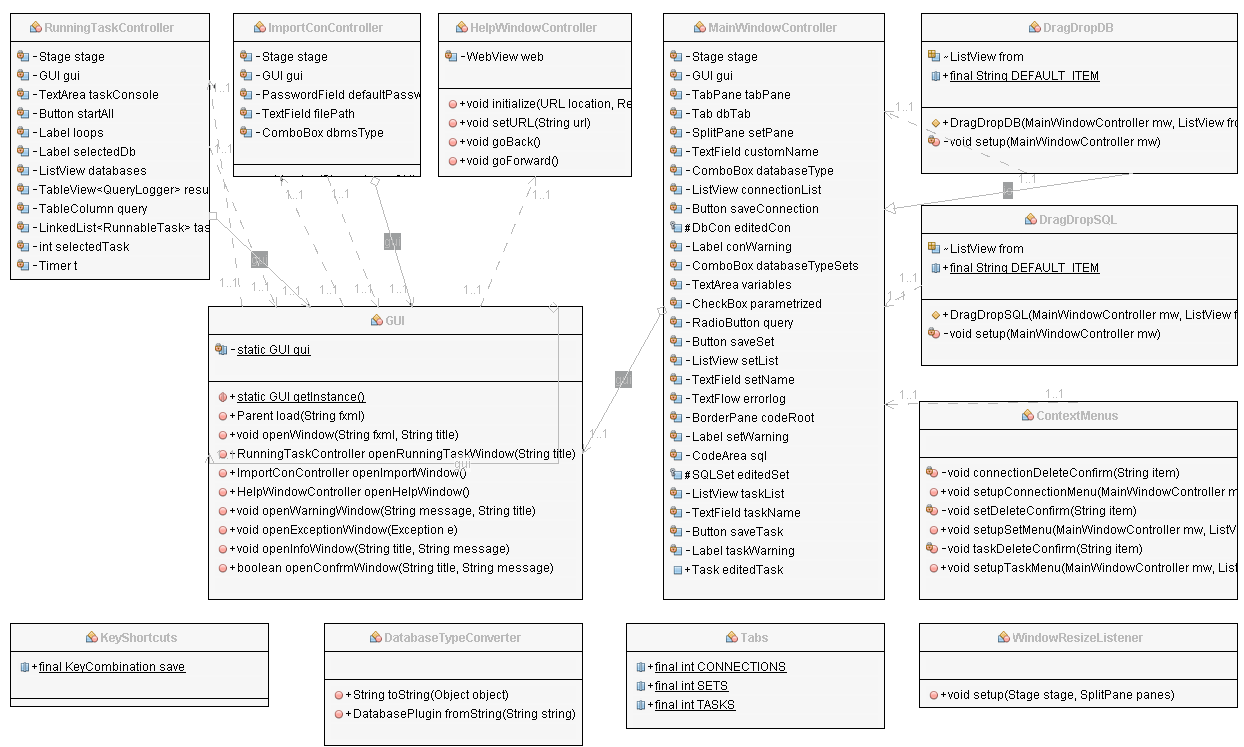
\includegraphics[width=1.0\textwidth]{Figures/PresentLayerDiagram.png}\caption{UML Diagram tříd prezentační vrstvy aplikace}
\end{figure}

Uživatelské rozhraní aplikace je definováno v FXML souborech. Tyto soubory jsou umístěny v balíku \textit{dbstresstest.gui.fxml}. Každý FXML soubor tvoří jedno okno aplikace a je mu přiřazena právě jedna JavaFX Controller třída pomocí argumentu \textit{fx:controller} v FXML souboru. Controller třída propojuje uživatelské rozhraní s logickou vrstvou aplikace, reaguje na akce uživatele a zpracovává události vyvolané během práce s grafickým rozhraním aplikace, pracuje tedy na pomezí prezentační a logické vrstvy.

Controller třída obsahuje referenci na všechny prvky uživatelského rozhraní, pomocí které lze k prvkům přistupovat a měnit jejich vlastnosti za běhu aplikace. Reference se předává do třídních proměnných jejichž název se musí shodovat s \textit{fx:id} prvku definovaného v FXML souboru. Reference na aktuální instanci prvku rozhraní JavaFX předává během inicializace controller třídy, aby předávání fungovalo, controller třída musí implementovat rozhraní \textit{javafx.fxml.Initializable}.

Aplikace celkem obsahuje 4 hlavní okna a k nim jsou přiřazeny 4 Controller třídy \newline \textbf{\emph{MainWindowController, RunningTaskController, HelpWindowController a ImportConController}}. Všechny Controller třídy mají vazby na Singleton třídu GUI, tato třída obsahuje pomocné funkce pro vyvolávání dodatečných dialogových oken. 

Třída \textbf{\emph{MainWindowController}} dále využívá pomocné třídy pro ovládání některých složitějších komponent. Třídy \textbf{\emph{DragDropDB}} a \textbf{\emph{DragDropSQL}} zajišťují funkcionalitu přetahování prvků sql a údajů k připojení k databázi v editoru úloh. Třída \textbf{\emph{ContextMenus}} vytváří kontextové nabídky v hlavním okně. V diagramu tříd prezentační vrstvy aplikace se dále nachází statické výčtové třídy \textbf{\emph{KeyShortcuts}} (obsahuje výčet klávesových zkratek) a \textbf{\emph{Tabs}} (obsahuje výčet záložek hlavního okna aplikace, jejich pořadí a jména).

\textbf{\emph{DatabaseTypeConverter}} rozšiřuje třídu \textit{javafx.util.StringConverter} a upravuje její funkcionalitu pro \textbf{\emph{DatabasePlugin}} třídy v naší aplikaci (viz. sekce \ref{plugins}).

Třída \textbf{\emph{WindowResizeListener}} reaguje na události spojené s změnou velikosti okna aplikace a přizpůsobuje tomu velikost některých grafických prvků. Jedná se především o ovládací prvky \textit{javafx.scene.control.SplitPane}, které ve výchozím stavu nereagují na změny velikosti okna a nezachovávají si proporční velikosti nastavené uživatelem. Třída se inicializuje společně s \textbf{\emph{MainWindowController}} třídou, tyto třídy tak na sebe nemají přímou vazbu.


\subsection{Hlavní okno aplikace}
Po spuštění aplikace je spuštěno hlavní grafické uživatelské rozhraní, to je rozděleno do tří podsekcí pomocí \textit{javafx.scene.control.TabPane}.

\newpage
\begin{figure}[!htbp]\centering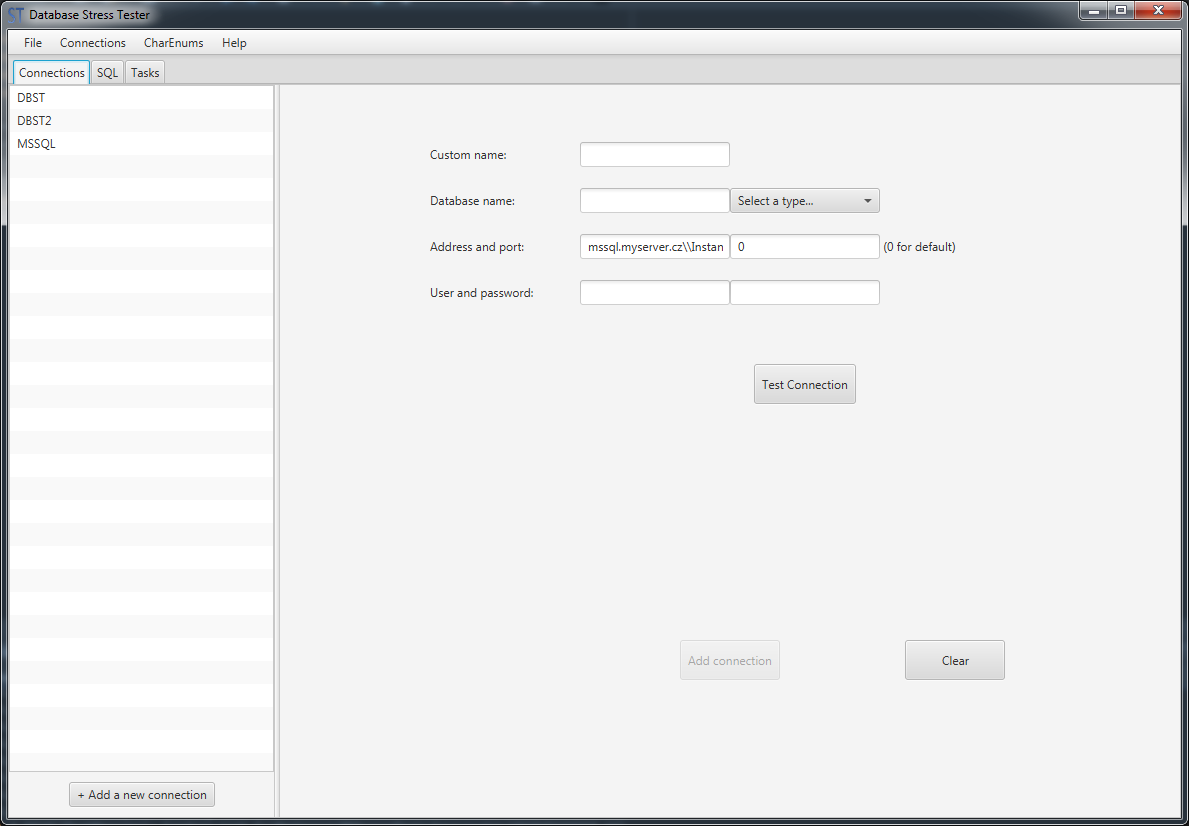
\includegraphics[width=1.0\textwidth]{Figures/coneditor.png}\caption{Okno editoru údajů k připojení k databázovému serveru}\label{coneditor}
\end{figure}
Okno editoru (obrázek \ref{coneditor}) pro správu údajů k připojení k databázovému serveru umožňuje přidávat nové položky pomocí tlačítka umístěného pod seznamem položek, nebo přes hlavní kontextovou nabídku aplikace. Existující položky lze editovat po kliknutí na jejich jméno v seznamu umístěného na levé straně okna. Pravým kliknutím na jméno položky, lze položku trvale odstranit. Samotný formulář odpovídá datové struktuře třídy \textbf{\emph{DbCon}} (viz. sekce \ref{datadiagram}). Heslo databázového uživatele se zadává do vstupního pole typu \textit{javafx.scene.control.PasswordField}, díky tomu se na monitor renderují pouze zástupné znaky \textbf{'•'}, místo skutečných znaků hesla.

Nad uloženými údaji lze provést test, tento test ověří, zda se k danému databázovému serveru lze připojit.

\newpage
\begin{figure}[!htbp]\centering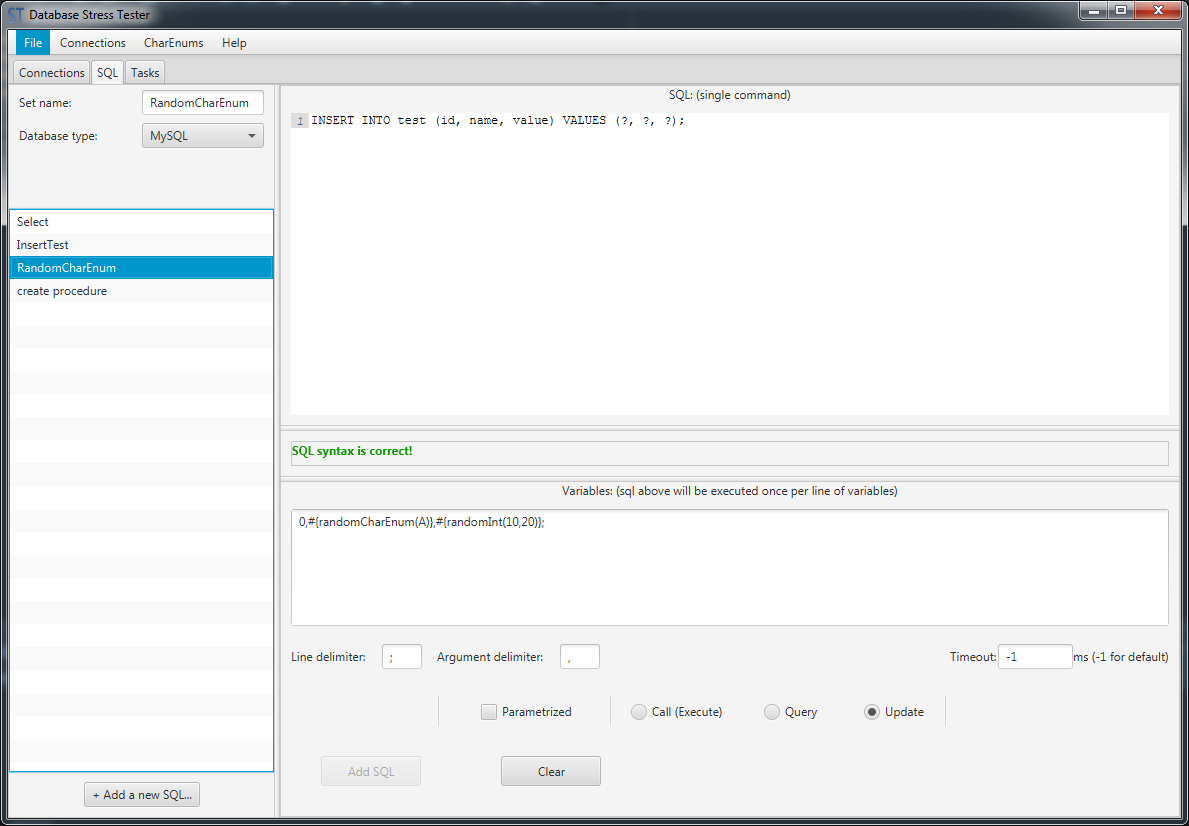
\includegraphics[width=1.0\textwidth]{Figures/sqleditor.png}\caption{Okno editoru SQL dotazů s parametry}
\end{figure}

TODO: popis

\newpage
\begin{figure}[!htbp]\centering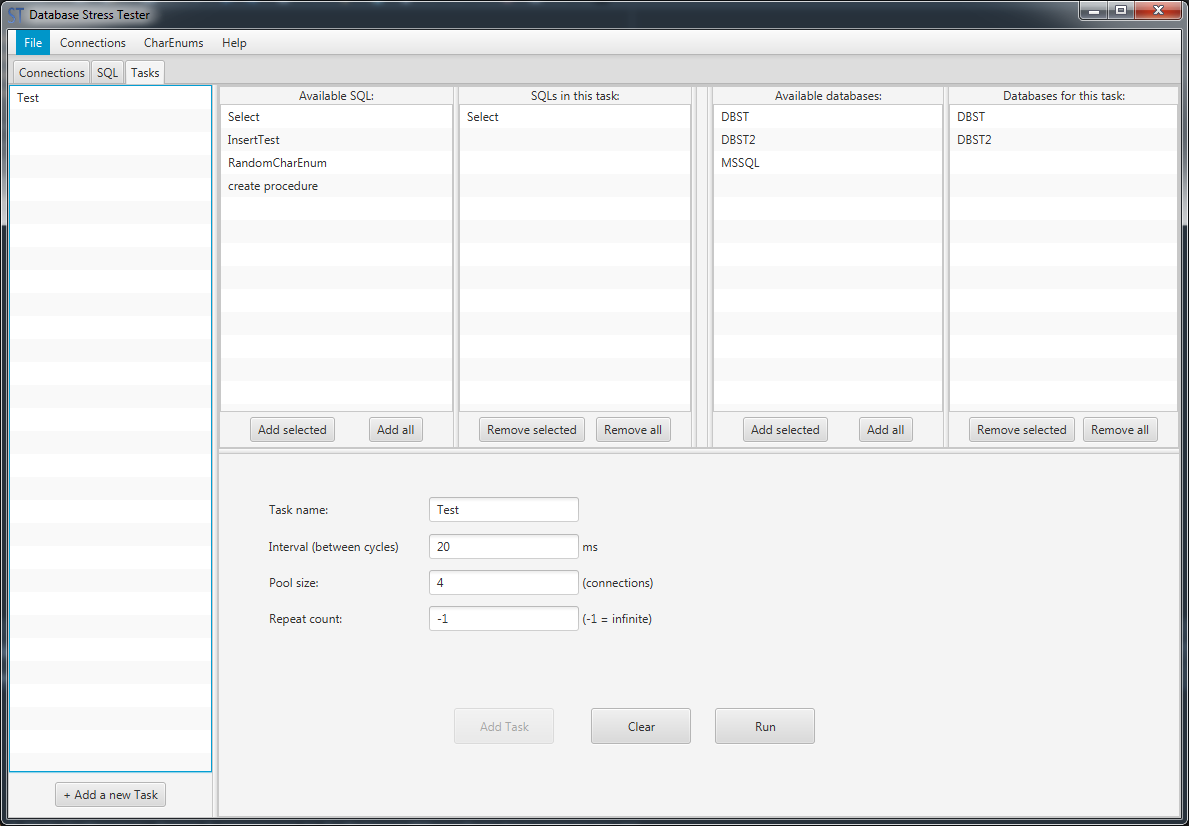
\includegraphics[width=1.0\textwidth]{Figures/taskeditor.png}\caption{Okno editoru spustitelných úloh}
\end{figure}

TODO: popis

\newpage
\subsection{Okno monitoru úloh}


\section{Logická vrstva} \label{logiclayer}
\subsection{Diagramy průběhu úlohy} \label{logic}
Pro popis logické vrstvy jsem zvolil sekvenční diagram, který bude pro popis operací vhodnější, než třídní diagramy, použité pro demonstraci struktury aplikace na datové a prezentační vrstvě. Následující sekvenční diagram demonstruje proces vytvoření spustitelné úlohy v aplikaci.

\begin{figure}[!htbp]\centering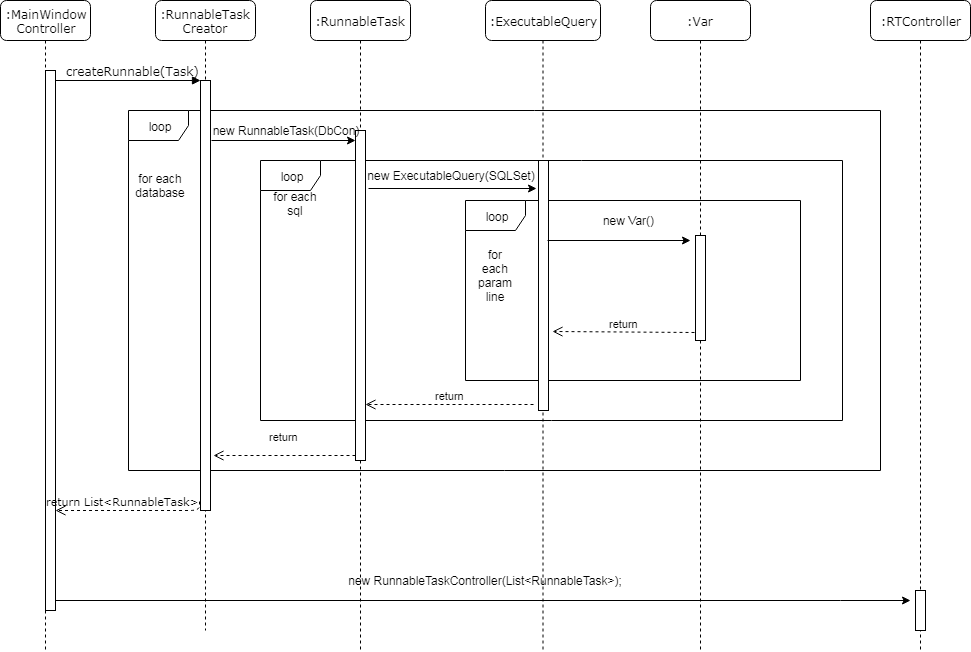
\includegraphics[width=1.0\textwidth]{Figures/rtprocess.png}\caption{Sekvenční diagram vytvoření spustitelné úlohy}
\label{seq1}
\end{figure}

\textbf{\emph{MainWindowController}} je třída na pomezí prezentační a logické vrstvy aplikace (viz. sekce \ref{prezent}). Po vyvolání události pro spuštění vybrané úlohy v prezentační vrstvě tato třída volá statickou metodu \textit{createRunnable(Task)} umístěnou ve statické třídě \textbf{\emph{RunnableTaskCreator}}, která vytvoří pole objektů \textbf{\emph{RunnableTask}}, pro každou databázi v této úloze je vytvořen právě jeden tento objekt.

Objekty typu \textbf{\emph{RunnableTask}} vytváří v konstruktoru sadu objektů, které implementují rozhraní \textbf{\emph{ExecutableQuery}} (implementace rozhraní se liší podle typu dotazu), pro každý samostatný SQL dotaz v dané úloze, je vytvořen právě jeden objekt. Pokud se jedná o parametrizovaný SQL příkaz, pak se pro každou sadu parametrů, se kterou se má dotaz spouštět, vytvoří pole objektů typu \textbf{\emph{Var}}. Tyto objekty zapouzdřují veškeré chování proměnných, rozpoznávají datové typy a vyhodnocují hodnoty funkcí.

Na konci diagramu je vytvořené pole objektů RunnableTask předáno v konstruktoru třídy  \textbf{\emph{RunnableTaskController}} (v diagramu zkráceno na \textit{RTController}). Daná úloha je v tuto chvíli připravena ke spuštění. Následující digram popisuje průběh úlohy.

\begin{figure}[!htbp]\centering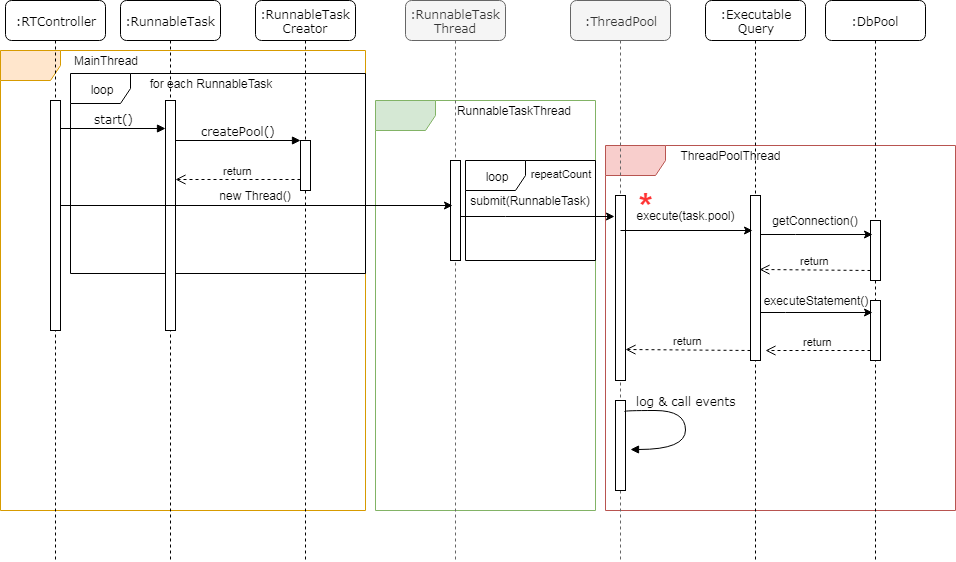
\includegraphics[width=1.0\textwidth]{Figures/runtask.png}\caption{Sekvenční diagram průběhu úlohy}
\label{seq2}

\textit{ThreadPool a RunnableTaskThread (označeny šedým pozadím) nejsou samostatné třídy, jsou součástí třídy \textbf{\emph{RunnableTask}}, v diagramu jsou zobrazeny na samostatných osách, aby bylo možné lépe popsat, operace prováděné na jednotlivých vláknech aplikace. }
\end{figure}


Diagram \ref{seq2} popisuje průběh spuštění úlohy od chvíle, kdy uživatel klikne na tlačítko start, tuto akci zachytí posluchač ve třídě \textbf{\emph{RunnableTaskController}} (v diagramu zkráceno na~\textit{RTController})~a~v~cyklu spustí úlohu pro všechny definované databáze v úloze metodou \textit{start()} volanou na objekty \textbf{\emph{RunnableTask}}, jejich vytvoření popisuje předchozí diagram \ref{seq1}. D8le je v rámci objektu \textbf{\emph{RunnableTask}} vytvořen objekt typu \textit{DbPool} pomocí statické třídy \textbf{\emph{RunnableTaskCreator}}, \textit{DbPool} je rozhraní, které definuje operace pro \textit{Connection Pool} (posloupnost předem vytvořených spojení s databázovým serverem). Implementace třídy \textit{DbPool} se liší v závislosti na typu databáze. Jednotlivé DBMS spravují samostatné rozšíření hlavní aplikace (viz. sekce \ref{plugins}).


Před samostatným spuštěním je ještě potřeba vytvořit Thread pool (posloupnost předem vytvořených vláken, v diagramu označeno jako \textit{ThreadPool}, pro implementaci je použit \newline \textit{java.util.concurrent.ExecutorService}), velikost je shodná s velikostí Connection poolu. Aby bylo možné zajistit funkcionalitu neomezeného počtu spuštění, které je ukončeno až akcí uživatele, je potřeba vytvořit další vlákno (v diagramu označeno jako \textit{RunnableTaskThread}, které bude časovat a odesílat jednotlivé SQL dotazy k vykonání do Thread Poolu pomocí metody \textit{submit(RunnableTask)} (Třída rozšiřuje rozhraní java.lang.Runnable a proto může být předána do \textit{ThreadPoolu}).













\subsection{Rozšíření aplikace} \label{plugins}

TODO:
zde popis jak fungují rozšíření aplikace




\newpage
\section{Validace SQL dotazů - SQL Lexer / Parser}
Jeden z cílů této práce je validovat SQL zadané uživatelem. Aby bylo možné zkontrolovat správnost zadaného SQL dotazu, potřebujeme znát kompletní gramatiku jazyka SQL a nad touto gramatikou postavit validátor (parser). Protože tohle téma je tak rozsáhlé, že by mohlo pokrýt celou samostatnou práci, použijeme na validaci SQL příkazů již existující knihovny. Před samotným výběrem knihovny, jsem prováděl testy volně dostupných knihoven pro zpracovávání SQL. Pro jazyk Java, co se volně dostupných knihoven týká, máme pouze 2 projekty, které jsou aktuální a stále se rozvíjí, projekt ANTRL a projekt jsqlparser.


\subsection{Projekt ANTLR (ANother Tool for Language Recognition)}
Projekt ANTRL je nástroj na čtení, zpracovávání, vykonávání nebo překládání strukturovaného textu nebo binárních souborů. Je velmi rozšířený pro budování jazyků, nástrojů a knihoven. ANTRL vygeneruje ze zadané gramatiky parser, který umožňuje sestavovat a procházet sestavené stromy ze zadané posloupnosti výrazů. \cite{antrl}



ANTRL využívá pro psaní gramatiky a parseru 2 soubory, aktuální verze ANTRL je 4, proto tyto soubory mají koncovku .g4. Soubor Lexer.g4 obsahuje veškerou gramatiku, kterou daný jazyk využívá, druhý soubor Parser.g4 obsahuje pravidla zpracovávaného jazyka. Jako jsou například posloupnosti klíčových slov jazyka a hodnoty mezi klíčovými slovy.
ANTRL z těchto souborů vygeneruje zdrojový kód v programovacím jazyce Java, nebo jiném, který požadujeme. Vygenerované zdrojové kódy poté použijeme v našem vlastním programu. \cite{antrldocs}



Výhoda ANTRL spočívá v tom, že gramatiky, které nabízí na oficiálních webových stránkách má umístěny na serveru github.com a gramatiky jsou tak otevřené k editaci pro širokou veřejnost vývojářů a případné chyby, které se v gramatice mohou objevit může opravit kdokoliv. ANTRL navíc nabízí gramatiky specifické pro různé verze jazyka SQL jako T-SQL, PL-SQL, MySQL a SQLite, které se liší především ve svých procedurálních rozšířeních. \cite{antrlg}



Největším problémem ANTRL je samotná práce programátora s vygenerovanými zdrojovými kódy, pokud se jedná o velmi rozsáhlý jazyk, jako je právě SQL. Pro jazyk Java a gramatiku pro PL-SQL ANTRL vygeneruje soubor PlSqlParser.java, který má více než 167 000 řádků kódu. Ve standardních vývojových prostředích pro jazyk Java, jako je například NetBeans IDE \ref{netbeans}, takto velký soubor nelze otevřít z důvodu nedostatku paměti, kterou nástroj potřebuje při načítání souboru.

\begin{table}[!htbp]
	\centering
	\caption{Počet řádků vygenerovaných zdrojových kódů ANTRL pro jazyk Java}
	\label{tab:parsers}
	\begin{tabular}{lllll}
		\toprule
		Parser & Lexer.java & Parser.java\\
		\midrule
		PL-SQL & 13 540 & 167 114 \\
        T-SQL & 4 611 & 98 484 \\
        MySQL & 5 108 & 60 411 \\
		\midrule
	\end{tabular}
\end{table}


Problémem existujících gramatik na oficiální github.com stránce projektu ANTRL je to, že k nim existuje pouze minimální nebo žádná dokumentace a tím, že každá gramatiku byla psána jinými lidmi, vznikají poté ve vygenerovaných zdrojových kódech odlišnosti. Například pokud chceme zobrazit stromovou strukturu SQL DML (Data Manipulation Language) dotazu, v každé gramatice je vygenerovaná metoda s odlišným názvem, kde \textit{parser} je reference na instanci parser třídy (tabulka \ref{tab:parsers}) vygenerované z dané gramatiky:\newline

\begin{lstlisting}[caption=T-SQL Parser]

parser.dml_clause().toStringTree();
\end{lstlisting}

\begin{lstlisting}[caption=PL-SQL Parser]

parser.data_manipulation_language_statements().toStringTree();
\end{lstlisting}

\begin{lstlisting}[caption=MySQL Parser]

parser.dmlStatement().toStringTree();
\end{lstlisting}

\newpage

\subsection{Testy ANTRL}
Právě díky tomu, že automaticky vygenerované třídy pomocí ANTRL jsou tak rozsáhlé, první vytvoření instance tříd v JVM je velmi pomalé, protože dochází k překladu Java kódu (bytecode). Opakované spouštění, nad již vytvořenými instancemi parser tříd, je již podstatně rychlejší, protože kód je již uložen v paměti JVM (v části paměti pojmenované jako \textit{Code Cache}), kde je uložen již přeložený Java kód (bytecode) na nativní strojový kód.

\begin{table}[!htbp]
	\centering
	\caption{ANTRL Test 1}
	Výsledky pro dotaz: 'SELECT * FROM TEST'
	\vskip 0.1cm
	\label{tab:antrl1}
	\begin{tabular}{lllll}
		\toprule
		Parser & První spuštění & Opakované spuštění & Správnost vyhodnocení\\
		\midrule
		PL-SQL & 1831 ms & 2 ms & Ano \\
        T-SQL & 525 ms & 1 ms & Ano \\
        MySQL & 428 ms & 1 ms & Ano \\
		\midrule
	\end{tabular}
\end{table}

\begin{table}[!htbp]
	\centering
	\caption{ANTRL Test 2}
	Výsledky pro dotaz: 'SELECT ** FROM TEST'
	\vskip 0.1cm
	\label{tab:antrl2}
	\begin{tabular}{lllll}
		\toprule
		Parser & První spuštění & Opakované spuštění & Správnost vyhodnocení\\
		\midrule
		PL-SQL & 1207 ms & 68 ms & Ano \\
        T-SQL & 416 ms &31 ms & Ne \\
        MySQL & 322 ms & 1 ms & Ne \\
		\midrule
	\end{tabular}
\end{table}

\begin{table}[!htbp]
	\centering
	\caption{ANTRL Test 3}
	Výsledky pro dotaz: 'SELECT COUNT(*) FROM TEST WHERE CID = 5 AND PRICE < 100 GROUP BY NAME ORDER BY PRICE'
	\vskip 0.1cm
	\label{tab:antrl3}
	\begin{tabular}{lllll}
		\toprule
		Parser & První spuštění & Opakované spuštění & Správnost vyhodnocení\\
		\midrule
		PL-SQL & 2556 ms & 5 ms & Ano \\
        T-SQL & 450 ms & 6 ms & Ano \\
        MySQL & 364 ms & 6 ms & Ano \\
		\midrule
	\end{tabular}
\end{table}

\begin{table}[!htbp]
	\centering
	\caption{ANTRL Test 4}
	Výsledky pro dotaz: 'SELECT COUNT(*) FROM TEST WHERE CID = 5 AND PRICE < 100 GROUP BY NAME ORDER PRICE'
	\vskip 0.1cm
	\label{tab:antrl4}
	\begin{tabular}{lllll}
		\toprule
		Parser & První spuštění & Opakované spuštění & Správnost vyhodnocení\\
		\midrule
		PL-SQL & 2522 ms & 6 ms & Ano \\
        T-SQL & 479 ms & 6 ms & Ne \\
        MySQL & 364 ms & 5 ms & Ano \\
		\midrule
	\end{tabular}
\end{table}


Z testů je vidět, že T-SQL a MySQL ANTRL parser nedokázal odhalit chybu ve špatné syntaxi dotazu \textit{SELECT ** FROM TEST} (viz. tabulka \ref{tab:antrl2}). T-SQL parser poté opakovaně selhal (viz.~tabulka~\ref{tab:antrl4}).



\subsection{Projekt Jsqlparser}
Projekt jsqlparser je postavený na knihovně JavaCC, která je vyvíjena samotnou společností Oracle. JavaCC je nástroj, který ze specifikace gramatiky dokáže vygenerovat zdrojové kódy v programovacím jazyce Java, umožňuje také sestavování stromové struktury jazyka pomocí nástroje JJTree, který je součástí JavaCC knihovny \cite{jsql}.


Nástroj Jsqlparser překládá dotaz jazyka SQL na ekvivalentní hierarchii Java tříd. Jsqlparser podporuje speciální SQL syntaxi pro Oracle, SqlServer, MySQL a PosgreSQL. Výsledek zpracovaného dotazu je možné strukturovaně procházet pomocí návrhového vzoru Visitor \cite{jsqld}.


\subsection{Testy Jsqlparser}
Pro možnost testy porovnat, jsou v testu použity stejné SQL dotazy, jako v předchozím testu ANTRL. Díky tomu, že Jsqlparser je univerzální a nemá gramatiky pro různé variace jazyka SQL nijak odděleny, nemůžeme porovnat rychlost zpracovávání dotazů pro PL-SQL, T-SQL a MySQL odděleně, jako v předchozím ANTRL testu. Pro měření opakovaného spouštění pro stejný dotaz bylo nutné použít v tomto testu měření v nanosekundách.

\begin{table}[!htbp]
	\centering
	\caption{JSqlparser test 1}
	Výsledky pro dotaz: 'SELECT * FROM TEST'
	\vskip 0.1cm
	\label{tab:jsql1}
	\begin{tabular}{lllll}
		\toprule
		Parser & První spuštění & Opakované spuštění & Správnost vyhodnocení\\
		\midrule
		Jsql & 30 ms & 0.26 ms & Ano \\
		\midrule
	\end{tabular}
\end{table}

\begin{table}[!htbp]
	\centering
	\caption{JSqlparser test 2}
	Výsledky pro dotaz: 'SELECT ** FROM TEST'
	\vskip 0.1cm
	\label{tab:jsql2}
	\begin{tabular}{lllll}
		\toprule
		Parser & První spuštění & Opakované spuštění & Správnost vyhodnocení\\
		\midrule
		Jsql & 29 ms & 0.34 ms & Ano \\
		\midrule
	\end{tabular}
\end{table}

\begin{table}[!htbp]
	\centering
	\caption{JSqlparser test 3}
	Výsledky pro dotaz: 'SELECT COUNT(*) FROM TEST WHERE CID = 5 AND PRICE < 100 GROUP BY NAME ORDER BY PRICE'
	\vskip 0.1cm
	\label{tab:jsql3}
	\begin{tabular}{lllll}
		\toprule
		Parser & První spuštění & Opakované spuštění & Správnost vyhodnocení\\
		\midrule
		Jsql & 33 ms & 0.59 ms & Ano \\
		\midrule
	\end{tabular}
\end{table}

\begin{table}[!htbp]
	\centering
	\caption{JSqlparser test 4}
	Výsledky pro dotaz: 'SELECT COUNT(*) FROM TEST WHERE CID = 5 AND PRICE < 100 GROUP BY NAME ORDER PRICE'
	\vskip 0.1cm
	\label{tab:jsql4}
	\begin{tabular}{lllll}
		\toprule
		Parser & První spuštění & Opakované spuštění & Správnost vyhodnocení\\
		\midrule
		Jsql & 33 ms & 0.75 ms & Ano \\
		\midrule
	\end{tabular}
\end{table}


\subsection{Srovnání parser knihoven}
Výsledky testování prokázaly, že JSqlparser bude pro naše účely vhodnější. Hlavním důvodem proč jsem pro jsem se rozhodl v aplikaci použít JSqlparser je fakt, že ANTRL parser vyhodnocuje dotaz při prvním spuštění více než vteřinu a v případě delších SQL dotazů až více než 2 vteřiny, jak ukazují předchozí testy. Taková doba je nepřijatelná, pokud chceme SQL validovat v reálném čase během doby, kdy uživatel SQL zadává do aplikace. Doba, kterou ANTRL parser vyžaduje, by způsobila pozastavení reakcí celé aplikace na akce uživatele během zadávání SQL dotazu, pokud by měla aplikace validovat SQL a v reálném čase zobrazovat výsledek. Díky rychlým odpovědím z JSqlParser je možné implementovat tento parser synchronně, ANTRL parser by vyžadoval asynchronní implementaci a výsledky by se zobrazovaly s prodlevou, výsledek validace by tak nemusel vždy odpovídat momentálnímu vstupu od uživatele.


































\section{Závěr}
TODO:


\begin{thebibliography}{99}
	\bibitem{antrl} Terence Parr. ANTLR (ANother Tool for Language Recognition) [online]. [cit. 2019-03-02]. Dostupné z: https://www.antlr.org/
	\bibitem{antrldocs} ANTRL Docs [online]. [cit. 2019-03-06]. Dostupné z: https://github.com/antlr/antlr4/blob/master/doc/index.md
	\bibitem{antrlg} ANTRL přehled dostupných gramatik [online]. [cit. 2019-03-02]. Dostupné z: https://github.com/antlr/grammars-v4
	\bibitem{jsql} The Java Parser Generator [online]. [cit. 2018-11-20]. Dostupné z: https://javacc.org/
	\bibitem{jsqld} JSql parser dokumentace [online]. [cit. 2019-03-10]. Dostupné z: https://github.com/JSQLParser/JSqlParser/wiki
	\bibitem{scenebuilder} Cindy Castillo. JSBGS.BOOK: JavaFX Scene Builder Getting Started with JavaFX Scene Builder Release 2.0 2014 [online]. [cit. 2019-03-10]. Dostupné z: https://docs.oracle.com/javase/8/scene-builder-2/JSBGS.pdf
	\bibitem{netbeans} A Brief History of NetBeans [online]. [cit. 2019-03-12]. Dostupné z: https://netbeans.org/about/history.html
	\bibitem{sqliso} Information technology -- Database languages -- SQL [online]. [cit. 2019-03-22]. Dostupné z: https://www.iso.org/standard/63555.html
	
	
	
	
	
\end{thebibliography}


\appendix % prilohy
\section{Zdrojový kód pro testování ANTRL - MySQL}
\begin{lstlisting}[caption=ANTRL MySQL]

	import antrl.mysql.MySqlParser;
	import antrl.mysql.MySqlLexer;
	import org.antlr.v4.runtime.*;

    static boolean mysqlresult = true;

    public static boolean mysql(String args) {
        mysqlresult = true;
        long start = System.currentTimeMillis();
        System.out.println("MySQL Check: " + args);
        CharStream stream = new ANTLRInputStream(args);
        MySqlLexer lexer = new MySqlLexer(stream);
        CommonTokenStream tokens = new CommonTokenStream(lexer);

        MySqlParser parser = new MySqlParser(tokens);

        parser.addErrorListener(new BaseErrorListener() {
            @Override
            public void syntaxError(Recognizer<?, ?> recognizer, Object offendingSymbol, int line, int pos, String msg, RecognitionException e) {
                System.out.println("Failed to parse at " + line + "," + pos + ":  " + msg);
                mysqlresult = false;
            }
        });
        parser.dmlStatement().toStringTree(parser);
        System.out.println("MySQL Result: " + mysqlresult + ", took: " + (System.currentTimeMillis()-start) + "ms");
        return mysqlresult;
    }
\end{lstlisting}
\section{Zdrojový kód pro testování ANTRL - T-SQL}
\begin{lstlisting}[caption=ANTRL T-SQL]

	import antrl.tsql.TSqlLexer;
	import antrl.tsql.TSqlParser;
	import org.antlr.v4.runtime.*;

  	static boolean tsqlresult = true;

    public static boolean tsql(String args) {
        tsqlresult = true;
        long start = System.currentTimeMillis();
        System.out.println("TSQL Check: " + args);
        CharStream stream = new ANTLRInputStream(args);
        TSqlLexer lexer = new TSqlLexer(stream);
        CommonTokenStream tokens = new CommonTokenStream(lexer);
        
        TSqlParser parser = new TSqlParser(tokens);

        parser.addErrorListener(new BaseErrorListener() {
            @Override
            public void syntaxError(Recognizer<?, ?> recognizer, Object offendingSymbol, int line, int pos, String msg, RecognitionException e) {
                System.out.println("Failed to parse at " + line + "," + pos + ":  " + msg);
                tsqlresult = false;
            }
        });
        parser.dml_clause().toStringTree(parser);
        System.out.println("TSQL Result: " + tsqlresult + ", took: " + (System.currentTimeMillis()-start) + "ms");
        return tsqlresult;
    }
\end{lstlisting}
\section{Zdrojový kód pro testování ANTRL - PL-SQL}
\begin{lstlisting}[caption=ANTRL PL-SQL]

	import antrl.plsql.PlSqlLexer;
	import antrl.plsql.PlSqlParser;
	import org.antlr.v4.runtime.*;

    static boolean plsqlresult = true;

    public static boolean plsql(String args) {
        plsqlresult = true;
        long start = System.currentTimeMillis();
        System.out.println("PLSQL Check: " + args);
        CharStream stream = new ANTLRInputStream(args);
        PlSqlLexer lexer = new PlSqlLexer(stream);
        CommonTokenStream tokens = new CommonTokenStream(lexer);

        PlSqlParser parser = new PlSqlParser(tokens);

        parser.addErrorListener(new BaseErrorListener() {
            @Override
            public void syntaxError(Recognizer<?, ?> recognizer, Object offendingSymbol, int line, int pos, String msg, RecognitionException e) {
                System.out.println("Failed to parse at " + line + "," + pos + ":  " + msg);
                plsqlresult = false;
            }
        });
        parser.data_manipulation_language_statements().toStringTree();
        System.out.println("PLSQL Result: " + plsqlresult + ", took: " + (System.currentTimeMillis()-start) + "ms");
        return plsqlresult;
    }
}
\end{lstlisting}


\section{Zdrojový kód pro testování JsqlParser}
\begin{lstlisting}[caption=ANTRL JSQL]
    public static boolean parse(String sql) {
        try {
            Statements st = CCJSqlParserUtil.parseStatements(sql);
            st.getStatements().get(0);
            return true;
        } catch (Exception ex) {
            System.out.println(ex.getCause().getMessage());
            return false;
        }
    }
\end{lstlisting}

\end{document}
